\chapter{Standard Model}

\label{ch:standardmodel}
% --------------------------------------------------------------------------------

The \SM of particle physics seeks to explain the symmetries and interactions of all currently discovered fundamental particles. 
It has been tested by several generations of experiments and has been remarkably succesful, no significant deviations have been found. 
The \SM provides predictions in particle physics for interactions up to the Planck scale (10\tsup{15}-10\tsup{19} GeV). 

The theory itself is a quantum field theory grown from an underlying $SU(3) \times SU(2) \times U(1)$ that requires the particle content and quantum numbers consistent with experimental observations (see Section~\ref{sec:particles}). 
Each postulated symmetry is accompanied by an interaction between particles through gauge invariance. 
These interactions are referred to as the Strong, Weak, and Electromagnetic forces, which are discussed in Section~\ref{sec:interactions}. 

Although this model has been very predictive, the theory is incomplete; for example, it is not able to describe gravity or astronomically observed dark matter. 
These limitations are discussed in more detail in Section~\ref{sec:limitations}. 

\section{Particles}
\label{sec:particles}

The most familiar matter in the universe is made up of protons, neutrons, and electrons. 
Protons and neutrons are composite particles, however, and are made up in turn by particles called quarks. 
Quarks carry both electric charge and color charge, and are bound in color-neutral combinations called baryons. 
The electron is an example of a lepton, and carries only electric charge. 
Another type of particle, the neutrino, does not form atomic structures in the same way that quarks and leptons do because it carries no color or electric charge. 
Collectively, these types of particles are known as fermions, the group of particles with half-integer spin. 

There are three generations of fermions, although familiar matter is formed predominantly by the first generation. 
The generations are identical except for their masses, which increase in each generation by convention. 
In addition, each of these particles is accompanied by an antiparticle, with opposite-sign quantum numbers but the same mass.

The fermions compromise what is typically considered matter, but there are additional particles that are mediators of interactions between those fermions.
These mediators are known as the gauge bosons, gauge in that their existance is required by gauge invariance (discussed further in Section~\ref{sec:interactions}) and bosons in that they have integer spin.
The boson which mediates the electromagnetic force is the photon, the first boson to be discovered; it has no electric charge, no mass, and a spin of 1.
There are three spin-1 mediators of the weak force, the two W bosons and the Z boson. 
The W bosons have electric charge of $\pm$ 1 and a mass of $80.385 \pm 0.015$ GeV, while the Z boson is neutral and has a mass of $91.1876 \pm 0.0021$ GeV. 
The strong force is mediated by eight particles called gluons, which are massless and electrically neutral but do carry color charge. 

The final particle present in the \SM is the Higgs boson, which was recently observed for the first time by experiments at CERN in 2012. 
It is electrically neutral, has a mass of $125.7 \pm 0.4$ Gev, and is the only spin-0 particle yet to be observed. 
The Higgs boson is the gauge boson associated with the mechanism that gives a mass to the W and Z bosons.

\begin{figure}[h]
  \centering
  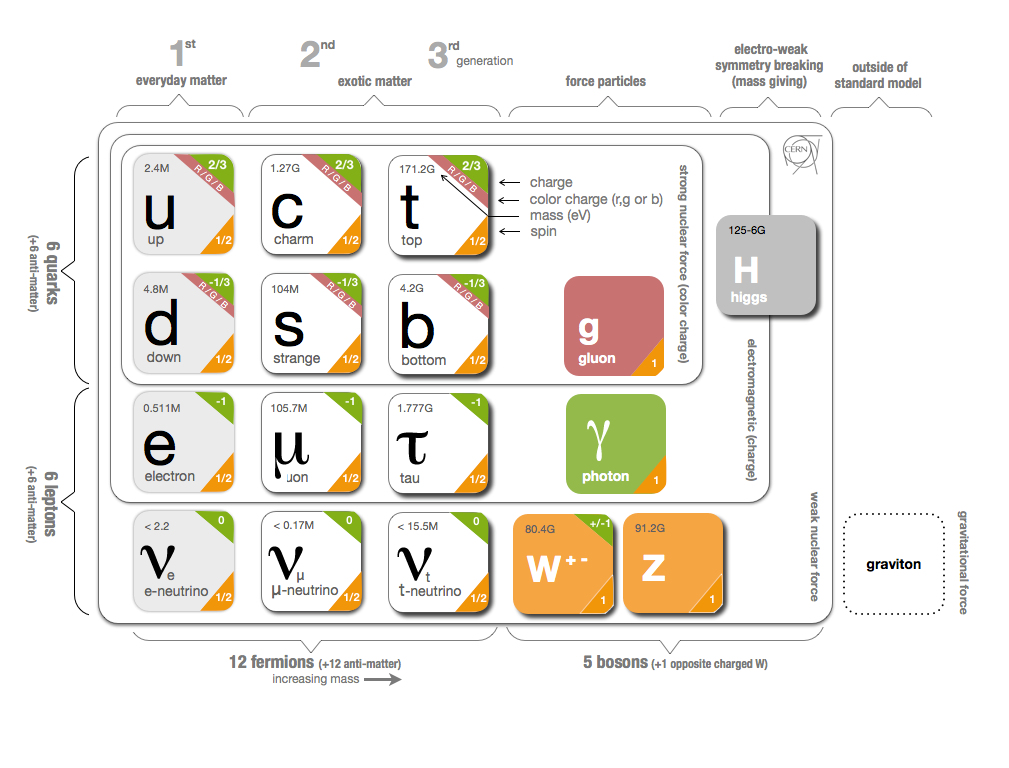
\includegraphics[width=0.9\textwidth]{figures/particle_content.png}
  \caption{The particle content of the \SM.}
  \label{fig:particle_content}
\end{figure}

Together these particles form the entire content of the \SM, and are summarized in Figure~\ref{fig:particle_content}. These are the particles that constitute the observable universe and all the so-far-observed interactions within it.


% ----------------------------------------

\section{Interactions}
\label{sec:interactions}

The interactions predicted and described by the \SM are fundamentally tied to the particles within it, both in that they describe the way those particles can influence each other and also in that the existence of the interactions requires the existence of some particles (the gauge bosons). 

% ----------------------------------------

\section{Limitations}
\label{sec:limitations}

% ----------------------------------------
